\documentclass[conference]{article}

% Packages for additional functionality
\usepackage[margin=.75in]{geometry}
\usepackage[utf8]{inputenc}
\usepackage{amsmath, amssymb}
\usepackage{graphicx}
\usepackage{algorithm}
\usepackage{algorithmic}
\usepackage[backend=biber,style=numeric,citestyle=ieee]{biblatex}
\usepackage{pdfpages}
\usepackage{subcaption}
\addbibresource{references.bib}

\title{\LARGE \bf
Final Report
}
\author{
    Jack Vranicar
}
\begin{document}
\maketitle

\thispagestyle{empty}
\pagestyle{empty}

\section{Abstract}

Typically, when selecting a spring, one can know with relative certainty what the spring constant will be. This is because the spring coefficient for certain spring designs and materials is well studied and characterized. However, if it is desirable to create an assembly solely with 3D printed parts, one will have difficulty applying these formulas. This is because it is difficult to reliably print a helical pattern with typical consumer grade 3D printers. To address this, an 'S' shaped spring model is introduced, and its response characterized. Sensitivity analysis is performed on this model to reduce the parameter set, and the results compared against a reference spring.
\section{Motivation}
% Describe the project to a layperson and include the statistaical mehtods you plan to use. Be clear on what params will be considered random params for UQ. This set may be reduced based on sensitivity analysis

\subsection{Mechanical Background}

For Mechanical Engineers, there are a number of considerations that must be made when designing a system, especially if it is a dynamic system. These dynamic systems have moving components and are subject to numerous external forces. To react to these external forces, there are a couple of schemes that are typically used. The first is passive control. This refers to a system that can react to disturbances appropriately, simply by virtue of its compliance and damping. There is also active control, which includes using actuators and sensors to effect the desired system response. Often, passive and active control schemes are used together to reap the benefits of both schemes. For the purposes of this analysis, only passive systems will be discussed.

When engineers are designing systems, it is typical to go through a number of iterations. This process helps make small changes to designs, compare iterations to each other and ending up with the best product. It is becoming increasingly popular to create these prototypes out of 3D printed materials as they allow for cheap, fast, and in-house manufacturing of all components. However, this approach is typically limited to static applications- parts that fasten to each other or do not require precise passive control considerations. One usually does not 3D print precise compliant parts due to the complexity of characterizing the spring's coefficients.  This can prove to be a serious limitation in a few cases, including a scale-model of a passively controlled system, or a passively controlled system that is intended to remain 3D printed. 

If a 3D printed spring could be precisely characterized, a number of benefits would become available to designers. The flexibility that printing one's own springs opens a wide variety of designs previously impossible with traditional methods. This can lead to innovative, novel solutions which can compensate for limitations of other designs. For this reason, the goal of this analysis is to determine a model which can reliably determine the spring constant and damping coefficient of a 3D printed spring.

\subsection{Statistical Background}

In order for a model to be useful, the parameters of the model must be identified. There are two strategies used to determine these parameters: frequentist and Bayesian approaches. Bayesian methods for parameter determination will be used in this discussion.

The Bayesian approach requires that one treats each parameter as a random variable, as opposed to the frequentist approach of treating each parameter as a fixed variable. This randomness is useful as it can account for uncertainties in production, such as measurement and manufacturing errors. Each of the parameters can then be defined as a Gaussian distribution with the mean value being the expected value of the error, and the variance representing the errors expected in producing the parameter. This is valuable for engineers as it allows for a better understanding of how these errors interact with each other and how confident they can be in the model prediction. 

However, it is not necessary or even desirable to treat every parameter of a system as if it is random. The first reason to fix a model parameter is if its value is known with high certainty. These could be the results of measurements with high-precision measurement tools. Another reason deals with identifiability. If a parameter is identifiable, that means that the Bayesian inference can be used to determine an expected value. However, in cases when parameters are unidentifiable, the inference cannot yield a conclusion on the expected value of the parameter. This typically happens when two or more parameters are a function of each other. This is because MCMC assumes that each of the parameters are independent and identically distributed (i.i.d.). If one parameter depends on the value of others, it is no longer i.i.d. Finally, fixing a parameter reduces the complexity of the modeling. Because the value for the parameter does not need to be sampled out of random distribution each time a point is evaluated, the MCMC requires less compute time. 

Two methods were used to determine which model parameters should be considered fixed: sensitivity analysis and MCMC. Sensitivity analysis is the process of quantifying how much a change in an input parameter changes the output parameters of the system. If a parameter is insensitive, it means that changing its value has little or no effect on the model's behavior. This is a means of determining that a parameter is unidentifiable as there is not definitive way of relating the parameter to the output of the system. % reference sensitivity analysis.

\subsection{Model Description}

Four of the parameters of this system describe its geometry Most of these parameters are displayed in Figure \ref{fig:SpringAnnotated}. A parameter not shown in \ref{fig:SpringAnnotated} is the Width $w$, which is the dimension into the page. This is a constant value for all of the components of the spring. Two more parameters, $\alpha$ and $E$, are included but do not relate to geometry. The definition of $\alpha$ is included in Equation \ref{eqn:kD}. $E$ is the measure of the Young's modulus for the spring.

The set of parameters $\theta$ that will be considered random variables for uncertainty quantification are the aforementioned parameters:

\begin{equation}
\theta =
	\begin{bmatrix}
		L & r & t & w & \alpha & E \\
	\end{bmatrix} ^T
	\label{eqn:OGParms}
\end{equation}

Below, this set is reduced using local sensitivity analysis. 

\begin{figure}[H]
    \centering
    \begin{subfigure}[t]{0.5\textwidth}
        \centering
	    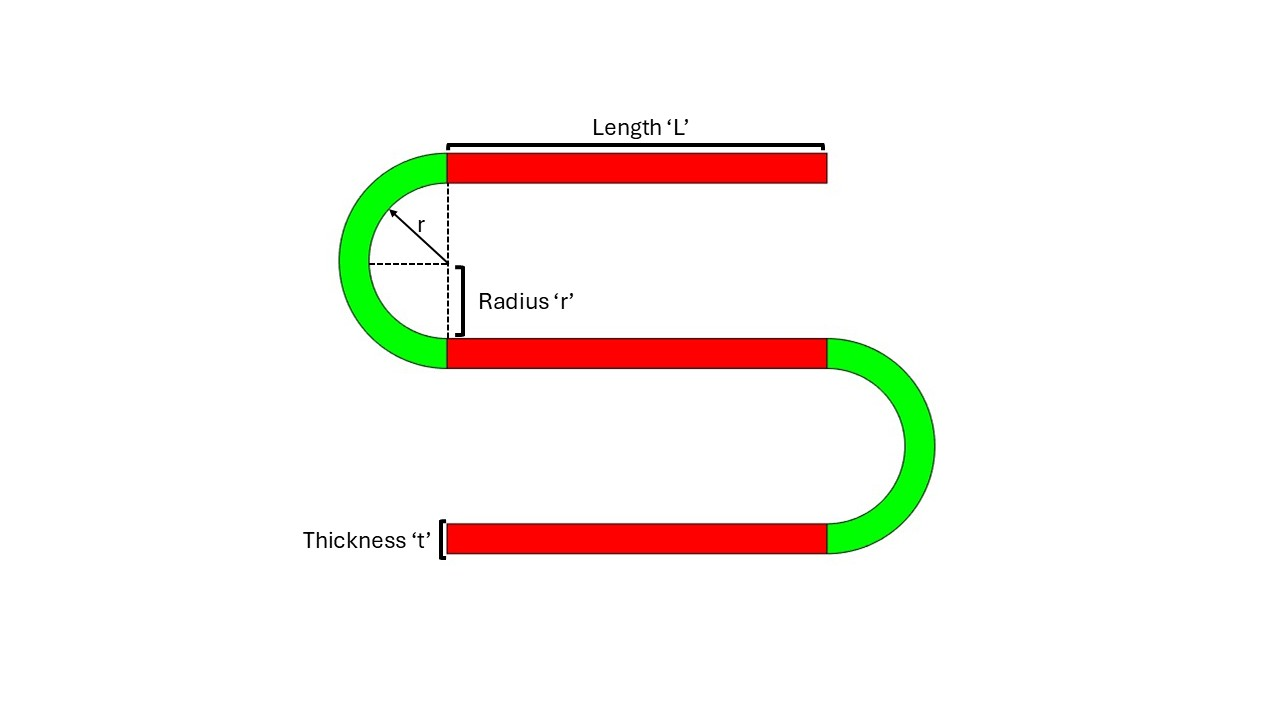
\includegraphics[width= \linewidth]{AnnotatedGraphic.jpg}
	    \caption{Spring Model: Uncompressed}
	    \label{fig:SpringAnnotated}
    \end{subfigure}%
    ~ 
    \begin{subfigure}[t]{0.5\textwidth}
       \centering
    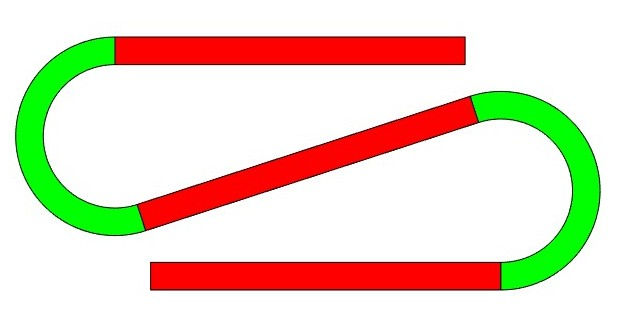
\includegraphics[width=\linewidth]{CompressedSpring.jpg}
    \caption{Spring Model: Compressed}
    \label{fig:SpringCompressed}
    \end{subfigure}
    \caption{Spring Model Compressed and Uncompressed}
\end{figure}



\subsection{Model Dynamics}

This system is modeled to behave as if it is a spring-mass-damper system. All of the mass is assumed to be concentrated at a point on the top of the spring. The damping is considered to be a linear function of velocity, and the stiffness is assumed to be a constant parameter based on physical and geometrical properties. Also, the system is assumed to have only one degree of freedom which is vertical displacement. 

The stiffness of this system is determined using the results derived by Wang et al. In this analysis, the characteristics of a micro-electro-mechanical system (MEMS) are determined through simulation and Finite Element Analysis (FEA). This MEMS structure is similar to the spring structure proposed in this analysis. The result of this analysis is that a stiffness matrix can be formed based solely on the properties of the materials and the shape of the MEMS structure. Because this derivation is quite complex, it will not be included. However, the stiffness matrix will herein be referred to as $\vec{K}$. \cite{mems}

Because this model is only using one degree of freedom, the effective spring constant can be extracted from $\vec{K}$ with the operation shown in Equations \ref{eqn:uK1} and \ref{eqn:uK2}. In Equation \ref{eqn:uK1}, $u$ represents a unit vector in the direction of the model's degree of freedom.

\begin{equation}
	u = \begin{bmatrix}
	1 & 0 & 0
	\end{bmatrix}^T 
	\label{eqn:uK1}
\end{equation}
\begin{equation}
	K_s = u^T \vec{K} u
	\label{eqn:uK2}
\end{equation}

The damping of this system was assumed to come only from drag. Typically, drag is a function of the square of velocity. This causes the model to be more complex due to nonlinearities. To reduce the complexity, a first order Taylor series approximation of the drag is taken. Because the velocity of the spring is relatively small, the reference point for this approximation is taken at a speed of zero. This approximation simplifies to the first-order time derivative of drag. Also, it is assumed that the drag will act in equal magnitude in both directions. Furthermore, a scaling term $\alpha$ is included to account for any unmodeled properties of the spring that contribute to drag. The damping coefficient used for the spring is shown below in Equation \ref{eqn:kD}.

\begin{equation}
	K_d = \alpha C_d \rho A
\label{eqn:kD}
\end{equation}

where $\rho$ is the density of air, and $A$ and $C_d$ are the cross-sectional area and coefficient of drag for the top surface of the spring, respectively.


\section{Analysis}
% Inlude an application of sensitivity (local or global) to understand if all parameters or some subset of parameters can be identified. Justify the type of sensitivity you use. This should be followed by an optimization of your random
% parameters (no UQ). 


\subsection{Optimization of Random Parameters}
To analyze the behavior of the model, a reference, or 'ideal,' spring-mass-damper system was created. Then, a genetic algorithm was used to best fit the parameters $\theta$ of the model to this ideal behavior. In both cases, a state-space model was utilized to predict the output of the springs. Because the springs are considered to be massless, the mass of the spring was applied as a constant input force to the system. The state vector $x$ is defined as: 
\begin{equation}
x = \begin{bmatrix}
y\\ \dot{y}\\
\end{bmatrix}
\end{equation}

where $y$ is the total height of the spring and $\dot{y}$ is the vertical velocity of the spring.\\

\noindent The following parameters A, B, C, and D were used to construct the state-space model:

\begin{equation}
A = \begin{bmatrix}
0 & 1 \\ -ks/m & -kd/m\\
\end{bmatrix}
\end{equation}

\begin{equation}
B = \begin{bmatrix}
0 & 1/m\\
\end{bmatrix}
\end{equation}

\begin{equation}
C = \begin{bmatrix}
1& 0\\
\end{bmatrix}
\end{equation}

\begin{equation}
D = \begin{bmatrix}
 0\\
\end{bmatrix}
\end{equation}

where $ks$ is the spring constant,  $kd$ is the damping coefficient, and  $m$ is the mass.

\subsubsection{Defining the Ideal Behavior}
\label{sec:Ideal}

To define the ideal behavior, the values $ks$, $kd$ and $m$ were defined as 200, 2, and 10, respectively. Then, using the aforementioned state-space model, the ideal height response was defined as shown in Figure \ref{fig:IdealResponse}. 

\subsubsection{Applying the Genetic Algorithm}
\label{sec:GA}

A genetic algorithm was applied to determine the optimal set of parameters to match the model to the ideal response. The cost function used for this algorithm was the Root Sum of Squares (RSS) of the model's response and the ideal spring's response. The set of parameters to achieve this fit was found to be:



\begin{equation}
	\theta_{opt} = \input{optimizedParams.tex}
\label{eq:ThOpt}
\end{equation}

\begin{figure}[H]
    \centering
    \begin{subfigure}[t]{0.5\textwidth}
        \centering
	    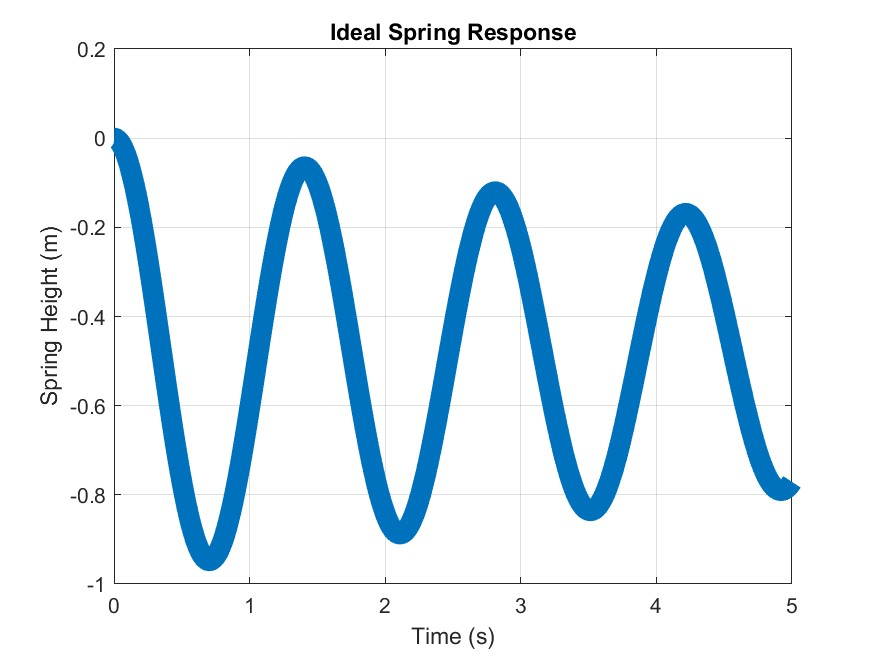
\includegraphics[width= \linewidth]{IdealSpringResponse.jpg}
	    \caption{Ideal Spring Response}
	    \label{fig:IdealResponse}
    \end{subfigure}%
    ~ 
    \begin{subfigure}[t]{0.5\textwidth}
       \centering
    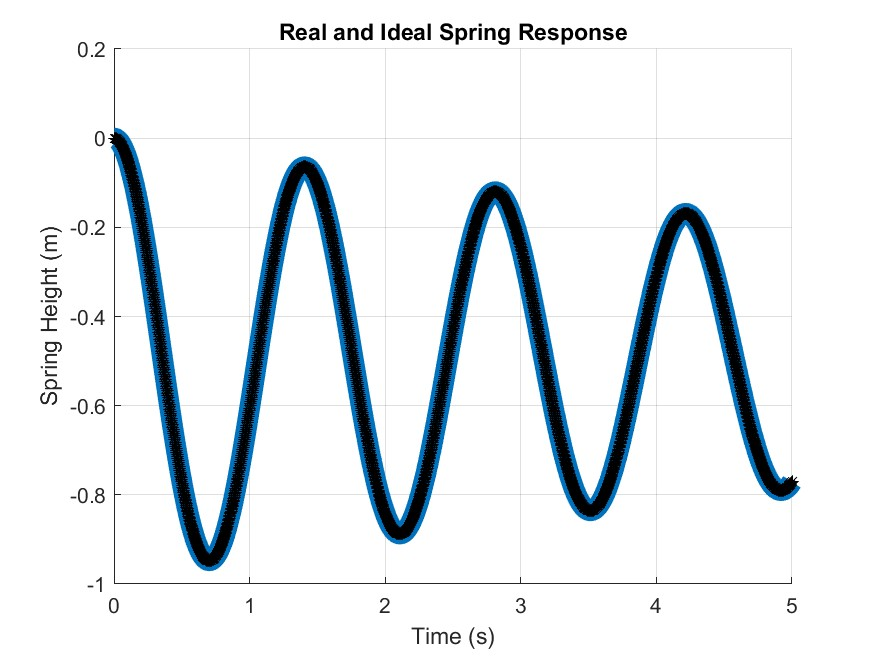
\includegraphics[width=\linewidth]{RealAndIdealSpringResponse.jpg}
    \caption{Model Response}
    \label{fig:SpringCompressed}
    \end{subfigure}
    \caption{Ideal and Model Responses}
\end{figure}

\subsection{Sensitivity Analysis}

The parameter set described in Equation \ref{eq:ThOpt} was used as the fixed point for sensitivity analysis using finite differerencing.

There are other optimized sets of model parameters, however these combinations tend to create a spring which is not feasible to manufacture, namely because they become very tall and thin. For this reason, local sensitivity was considered to be appropriate to avoid entering these regions.

Furthermore, finite differencing was utilized as the computational load of the model is small and this method is naive to the system's dynamics. This allows for fine tuning of the model in the future without affecting the efficacy of the sensitivity analysis. Complex step method was not utilized due to the unstable affects of using complex number to define dimensions.

Starting at the fixed point, each model parameter was perturbed using finite differencing. A scaled distance $\Delta$ is defined for each model parameter $\theta_{opt}^i $ such that the maximum value is $\theta_{opt}^i +  \Delta \theta_{opt}^i  $ and the minimum value is  $\theta_{opt}^i  -  \Delta \theta_{opt}^i  $ . By repeating this process over multiple test points for each model parameter, an approximation of the Jacobian of the model near the fixed point is defined as $S$. Each of these sensitivities is plotted against the test points that were used, as shown in Figure \ref{fig:LocalSens}.

\begin{figure}[H]
    \centering
    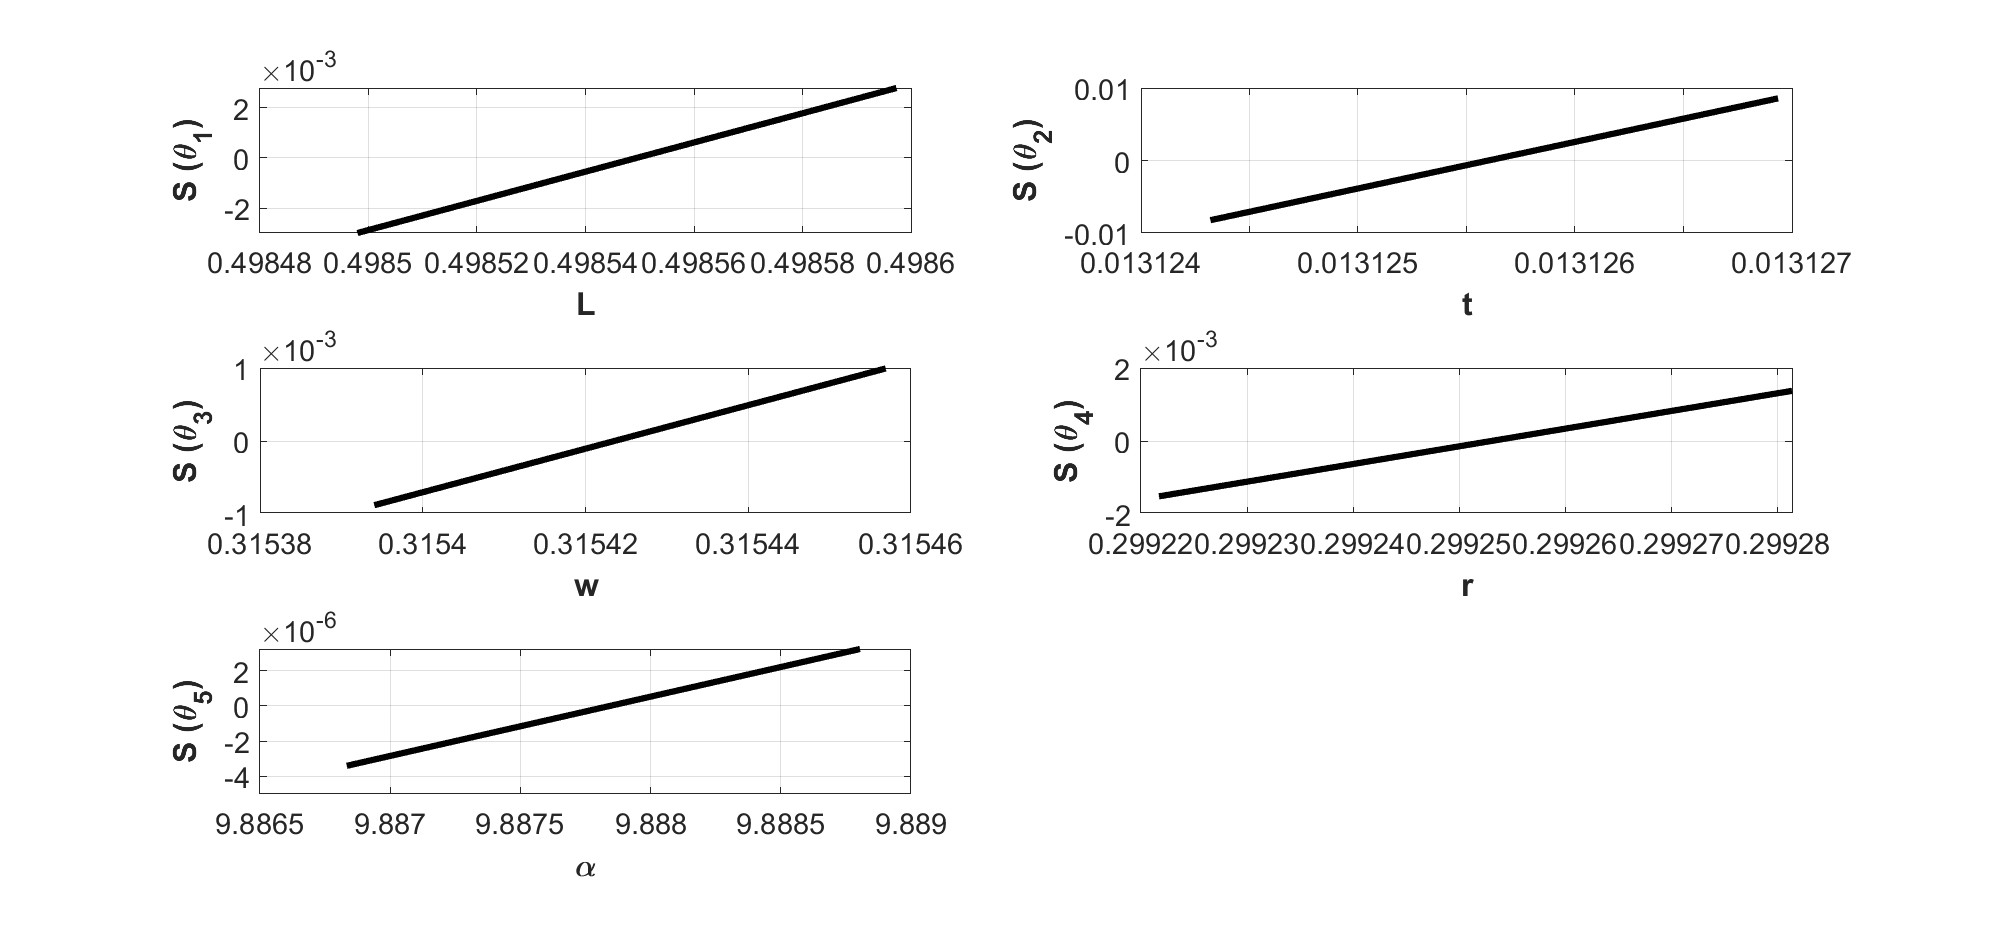
\includegraphics[width= .8\linewidth]{LocalSens.jpg}
    \caption{Local Sensitivities}
    \label{fig:LocalSens}
 \end{figure}
 
 From Figure \ref{fig:LocalSens}, it can be concluded that $\theta_1$ is insensitive and therefore is unidentifiable. For this reason, the parameter set, defined in Equation \ref{eqn:OGParms}, can be reduced to:
 
 \begin{equation}
\theta_{RED} =
	\begin{bmatrix}
		r & t & w & \alpha \\
	\end{bmatrix} ^T
	\label{eqn:RedParms}
\end{equation}
 
 Using the genetic algorithm described in Section \ref{sec:GA}, this reduced set of parameters was optimized. Figure \ref{fig:OptFit} below shows the results of this parameter fitting.
 
 \begin{figure}[H]
    \centering
    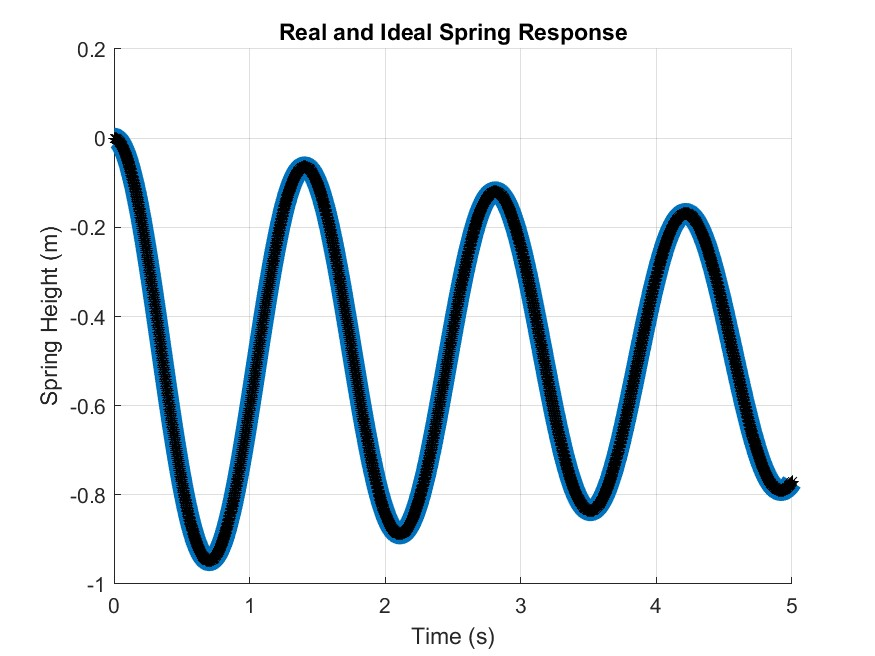
\includegraphics[width=.75  \linewidth]{Reduced_RealAndIdealSpringResponse.jpg}
    \caption{Model Fitting with $\theta_{RED}$}
    \label{fig:OptFit}
 \end{figure}
 
\section{Uncertainty Quantification}
% Four plots. Make sure theta is defined

Uncertainty quantification for each of the parameters in the full set and the reduced set was conducted using MCMC methods. 

% Full Set

 \begin{figure}[H]
    \centering
    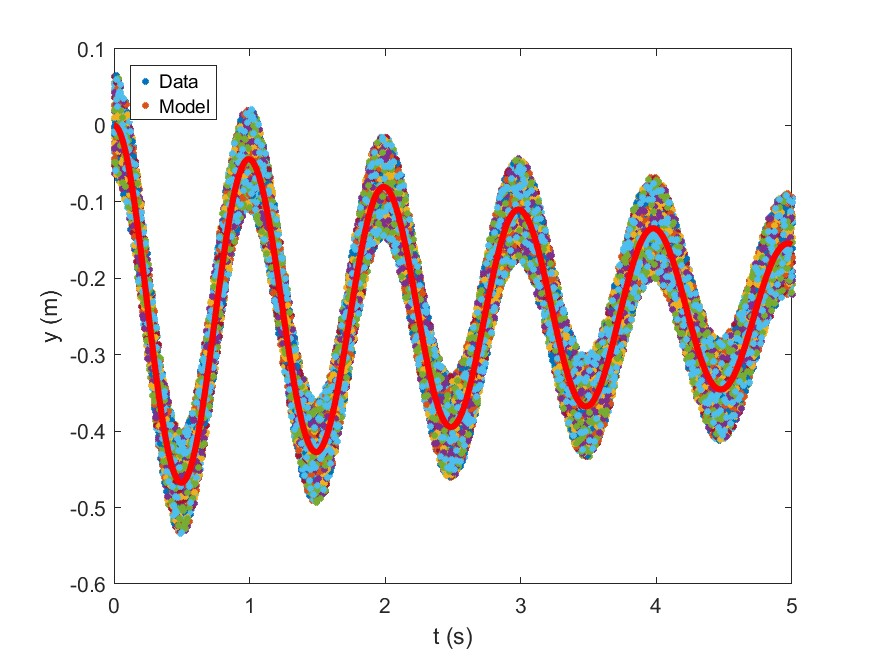
\includegraphics[width=.75  \linewidth]{FullParamSetInitialGuess.jpg}
    \caption{Model Fitting with $\theta_{RED}$}
    \label{fig:OptFit}
 \end{figure}
 
 \begin{figure}[H]
    \centering
    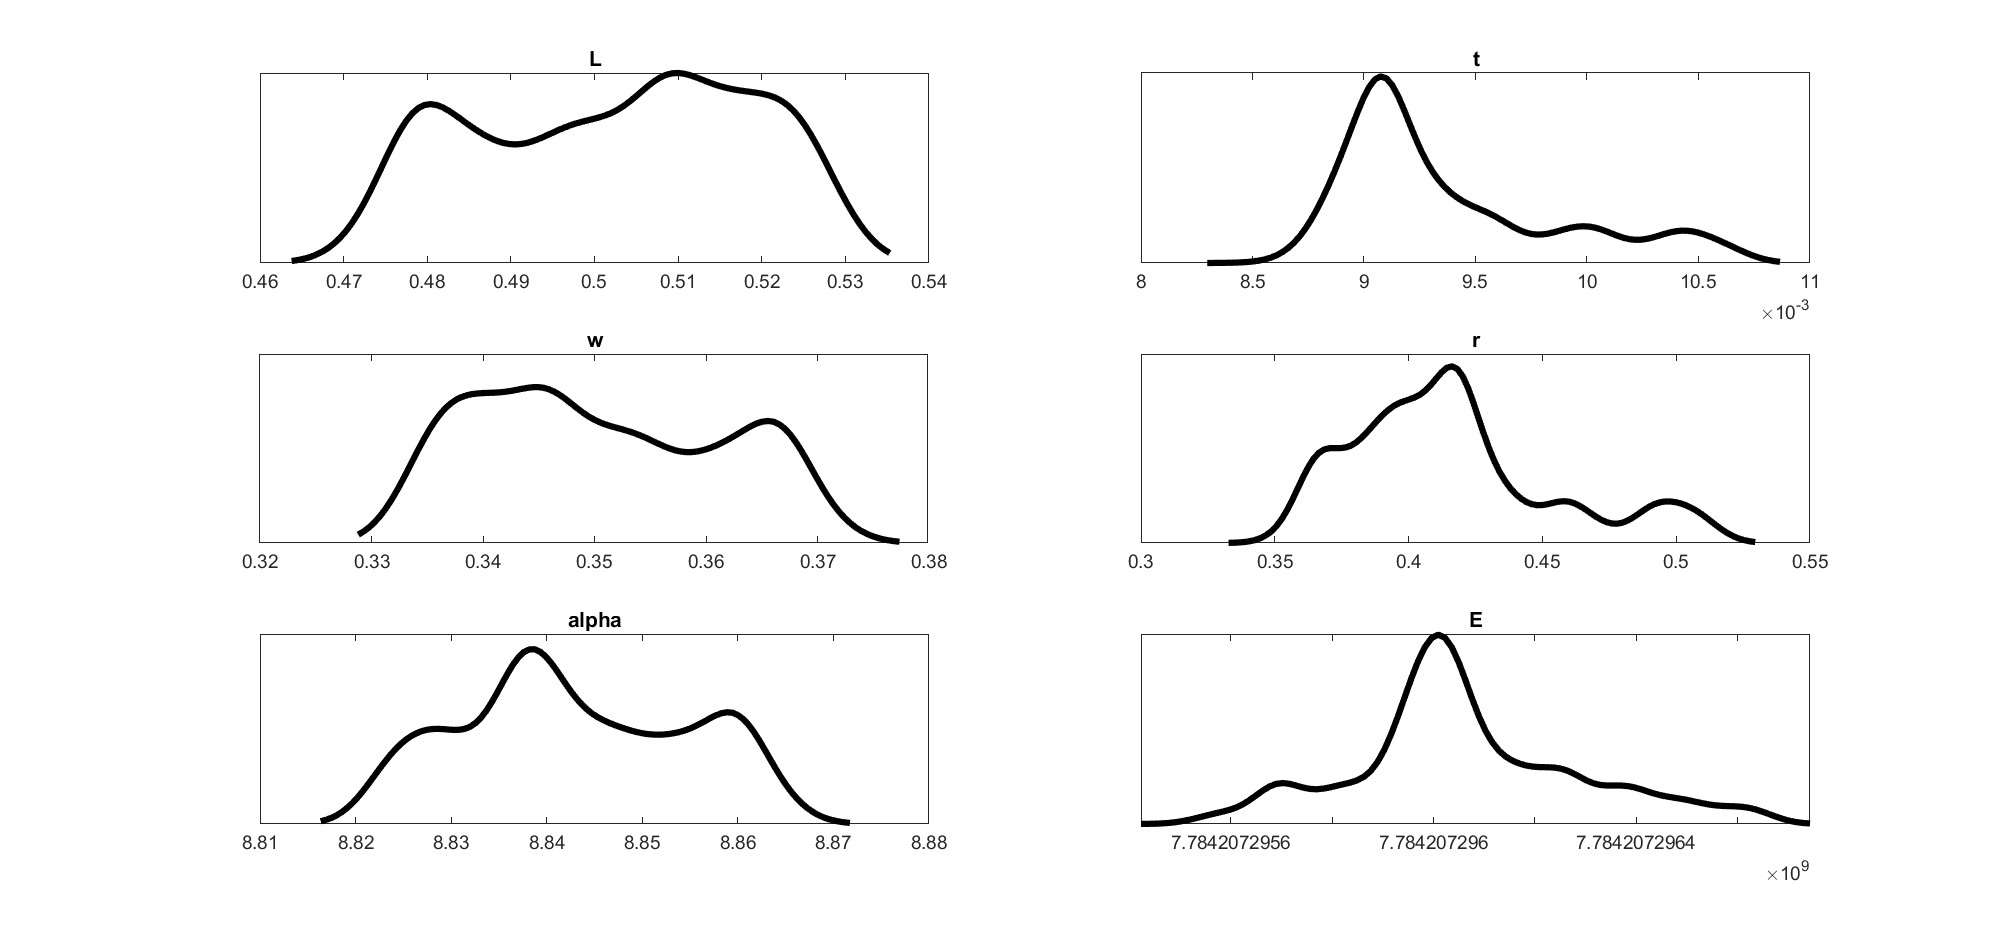
\includegraphics[width=.75  \linewidth]{FullParamSetChains.jpg}
    \caption{Model Fitting with $\theta_{RED}$}
    \label{fig:OptFit}
 \end{figure}
 
 \begin{figure}[H]
    \centering
    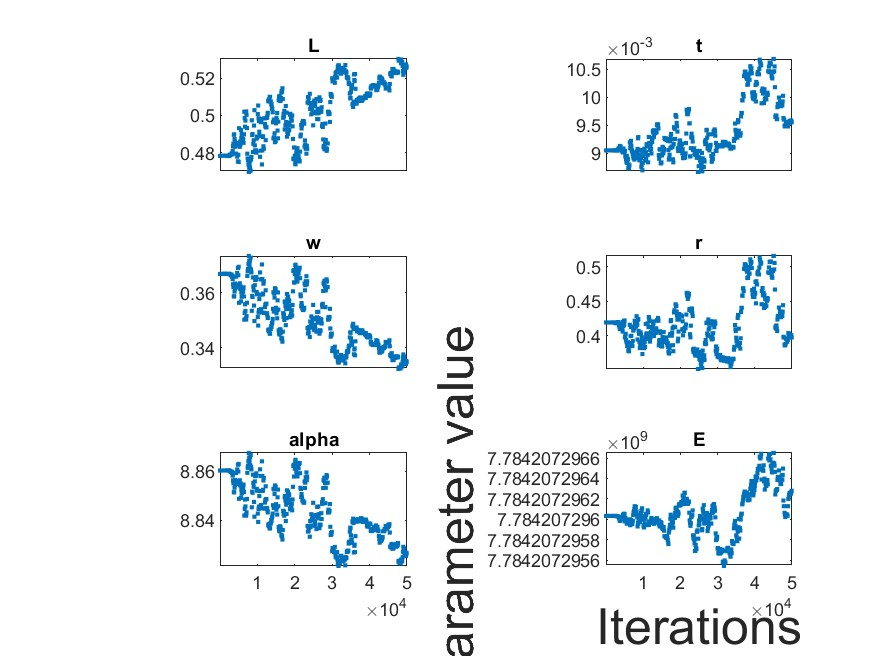
\includegraphics[width=.75  \linewidth]{FullParamSetChainPanel.jpg}
    \caption{Model Fitting with $\theta_{RED}$}
    \label{fig:OptFit}
 \end{figure}
 
 \begin{figure}[H]
    \centering
    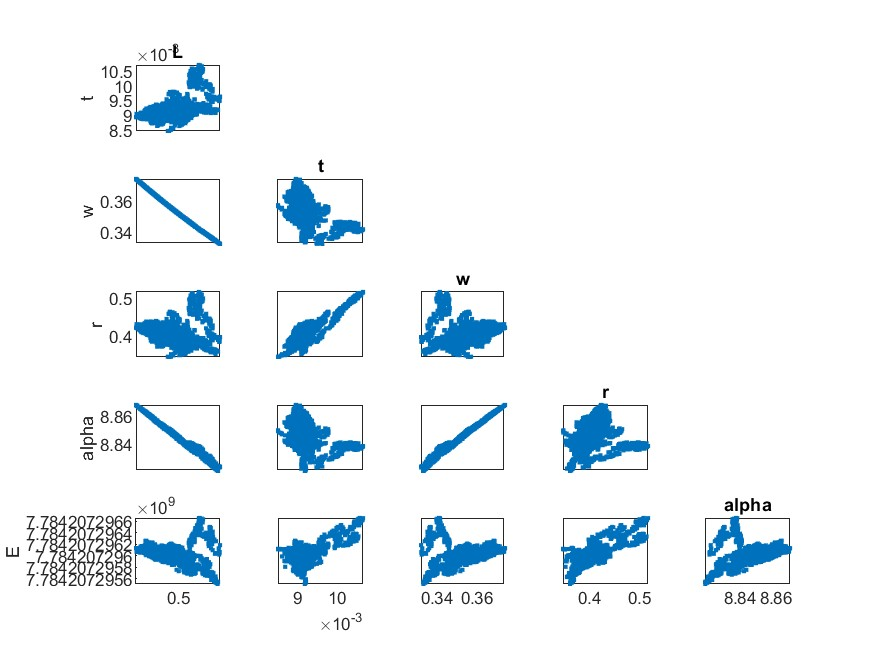
\includegraphics[width=.75  \linewidth]{FullParamSetPairs.jpg}
    \caption{Model Fitting with $\theta_{RED}$}
    \label{fig:OptFit}
 \end{figure}

% Reduced set
\begin{figure}[H]
    \centering
    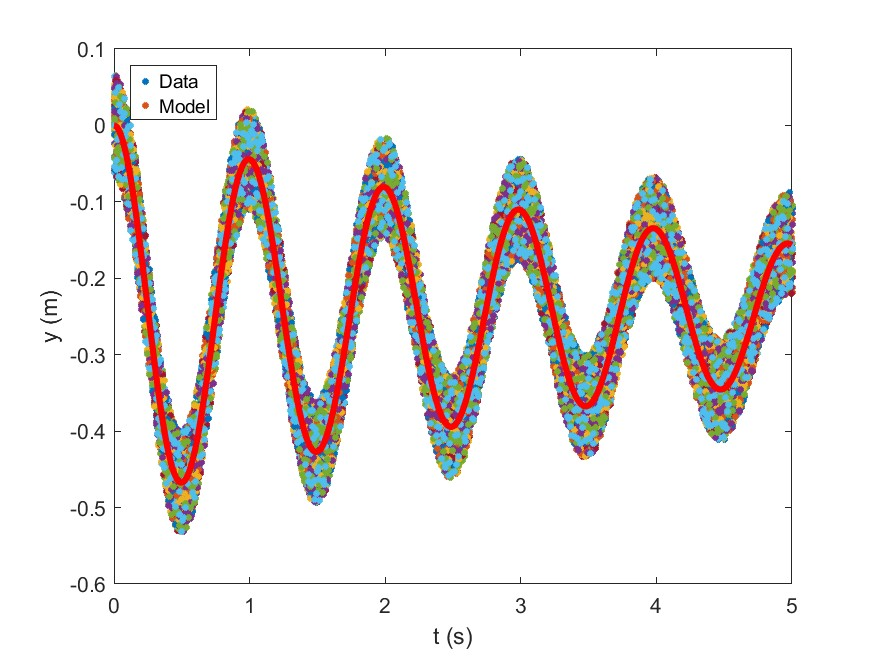
\includegraphics[width=.75  \linewidth]{RedParamSetInitialGuess.jpg}
    \caption{Model Fitting with $\theta_{RED}$}
    \label{fig:OptFit}
 \end{figure}
 
 \begin{figure}[H]
    \centering
    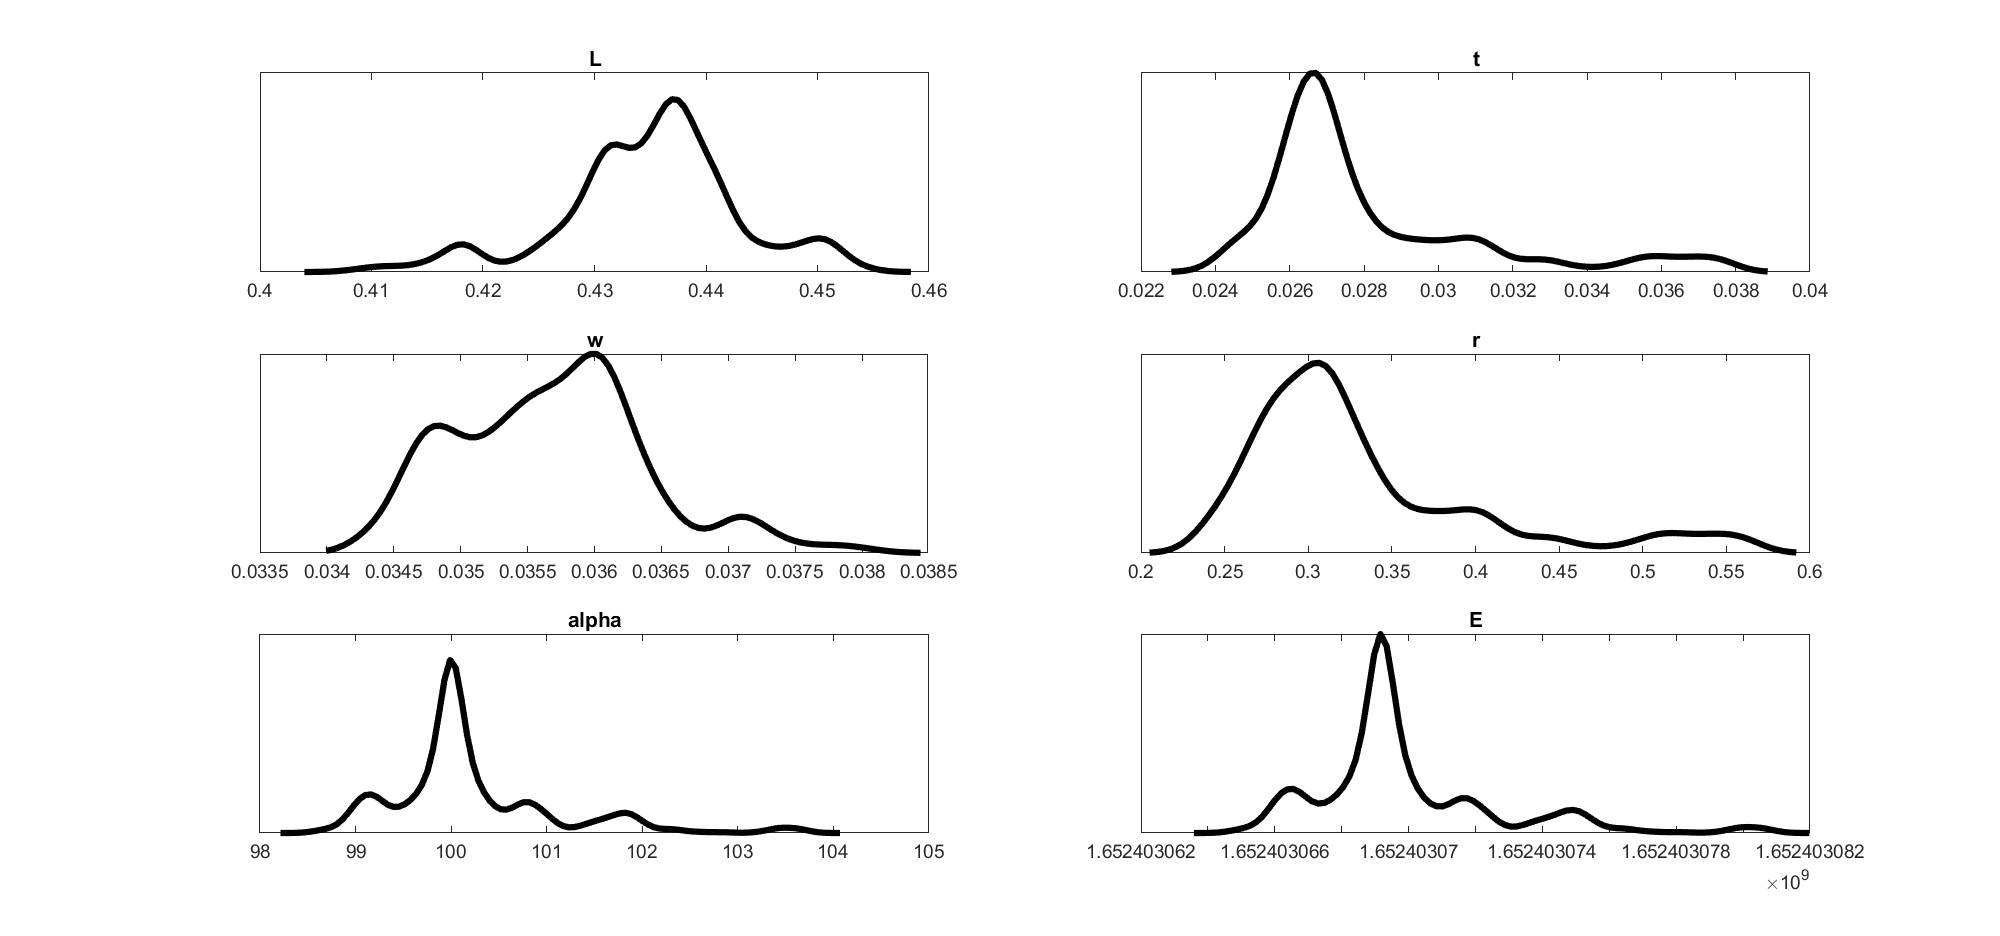
\includegraphics[width=.75  \linewidth]{RedParamSetChains.jpg}
    \caption{Model Fitting with $\theta_{RED}$}
    \label{fig:OptFit}
 \end{figure}
 
 \begin{figure}[H]
    \centering
    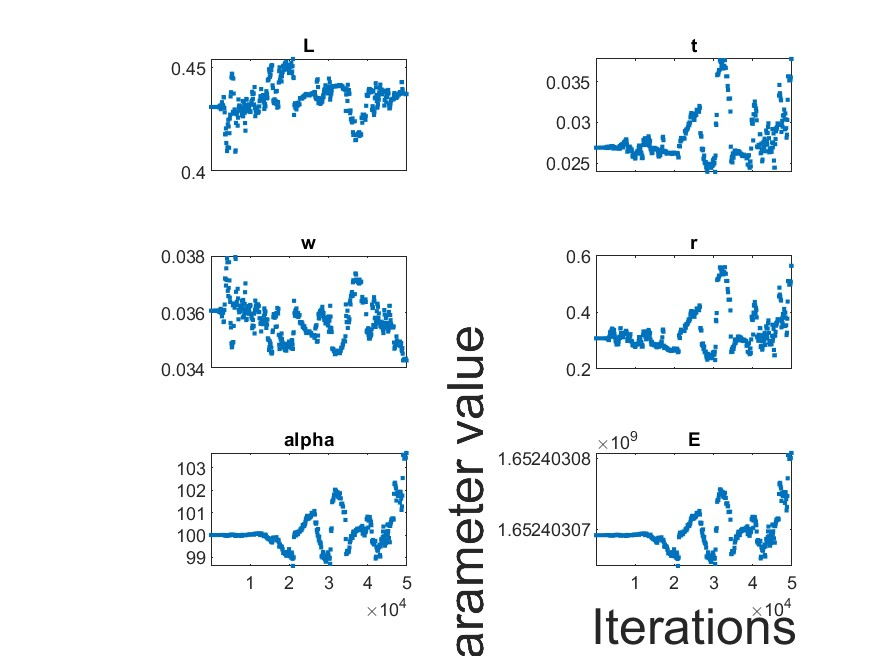
\includegraphics[width=.75  \linewidth]{RedParamSetChainPanel.jpg}
    \caption{Model Fitting with $\theta_{RED}$}
    \label{fig:OptFit}
 \end{figure}
 
 \begin{figure}[H]
    \centering
    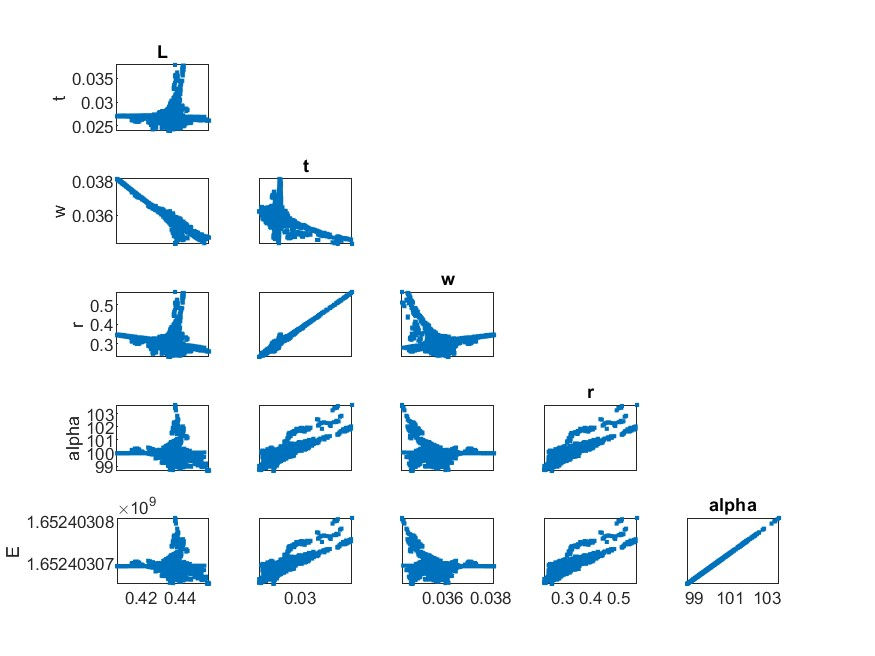
\includegraphics[width=.75  \linewidth]{RedParamSetPairs.jpg}
    \caption{Model Fitting with $\theta_{RED}$}
    \label{fig:OptFit}
 \end{figure}


\section{Concluding Remarks}
% Key findings. How did parameters affect QoI?

\newpage
\printbibliography


\end{document}

\subsection{Proposed Statistical Methods}
% Write about monte carlo

%In the future, uncertainty quantification will be performed on this system to quantify each of the system parameters. To do this, Markov Chain Monte Carlo (MCMC) sampling will be applied. This method is selected as it allows parameter uncertainty to be determined for all parameters. Also, MCMC will help to explore a wide range of combinations for each of the parameters. This is necessary for this model as optimizations have demonstrated a number of modes for spring parameters. These modes include springs that have: very large $r$ and $t$ values but very small $L$ values; very large $r$ and $L$ values but very small $t$ values; and balanced $r$ $L$, and $t$ values. For each of these modes, the value of $w$ is typically very small. By exploring the entire parameter space, it may be possible to find equivalent springs that are constructed in different modes, allowing for more flexibility in design.
%
%To simulate measurement noise and dimensional errors in the spring's construction, Gaussian noise will be added to each of the sample points of candidate springs used when matching the model to the ideal spring. 
